\chapter{Framework}
This chapter presents an overview of the proposed data cleaning framework. 
The framework is designed to clean raw tabular datasets by combining statistical data profiling techniques with LLMs that generate executable cleaning code.
Each component of the framework is described and analyzed in detail, with Figure \ref{fig:framwork_architecture} illustrating the overall architecture.

\begin{figure}[h]
    \centering
    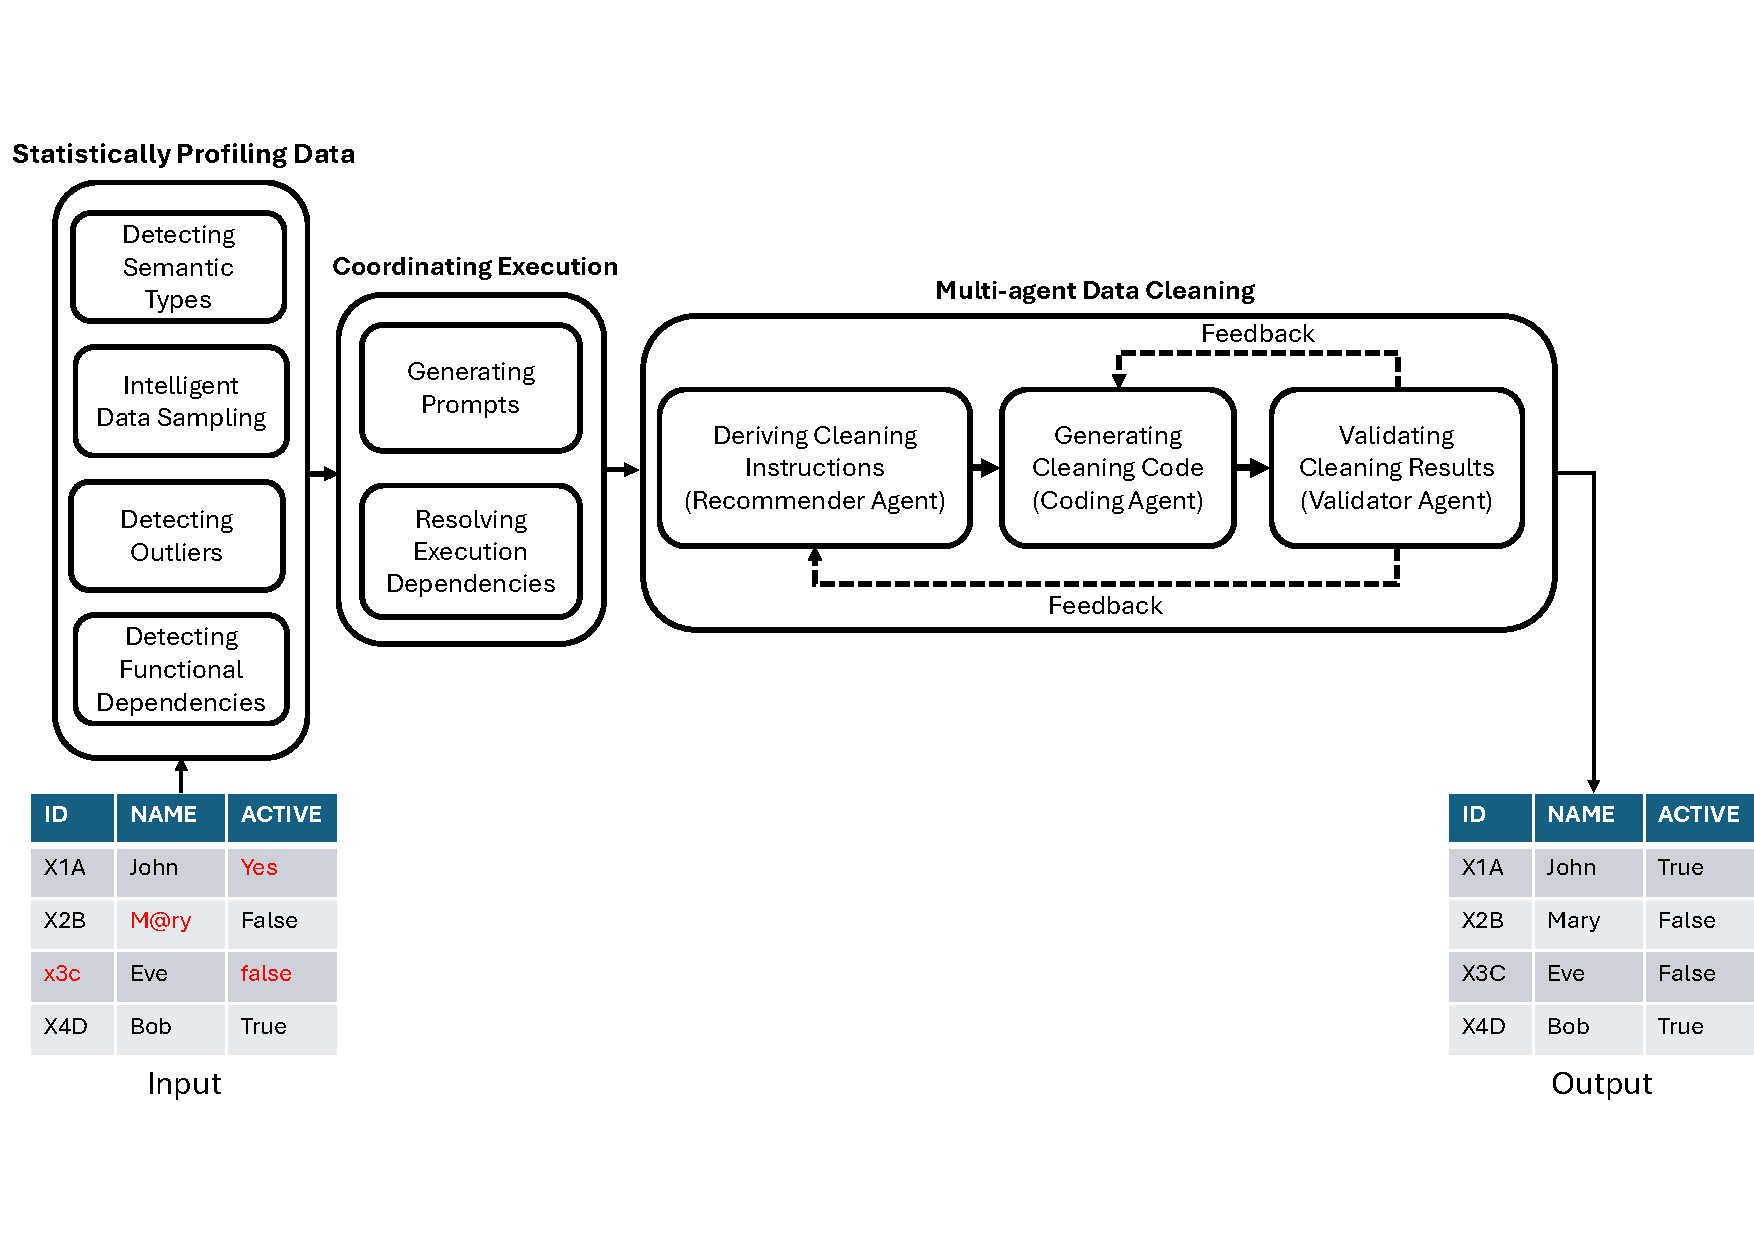
\includegraphics[width=0.95\linewidth]{Figures/framework_fig.pdf}
    \caption{DRAFT! Proposed Framework Architecture}
    \label{fig:framwork_architecture}
\end{figure}

\section{Data Profiler}
A major challenge when using LLMs for data cleaning is that they cannot process entire datasets at once due to limited context windows. 
While one could batch smaller parts of a dataset and process them sequentially, this approach does not scale well for large datasets, as it leads to increased runtime and token usage. 
In addition, as discussed before, LLMs generally struggle to identify statistical patterns in numerical data, especially when handling large, noisy or repetitive numeric datasets.
\newline\newline
Instead of directly passing raw tabular data to the LLM, the proposed framework first applies statistical and rule-based profiling techniques to summarize the data. 
The goal is to reduce noise, highlight relevant patterns and errors, and provide the LLM with compact but informative representations of the data. 
Furthermore, each column is assigned a predefined semantic type, which allows the framework to adapt the cleaning strategy to the characteristics of the data. 
Together, these steps enable the LLM to reason at the column level and generalize cleaning operations across the entire column, rather than relying on cell-level examples.
\newline\newline
Raw tabular datasets can be provided to the framework in common formats CSV, XLSX and JSON. 
Once loaded into the framework, the dataset is passed to the Data Profiler, which analyzes the data and produces a structured profile. 
The dataset is cleaned in a column-wise fashion, meaning that each column is processed independently in the initial stages. 
For this reason, the Data Profiler creates a separate profile for each column. 
This column-level focus is central to the framework design, as it allows the system to capture the specific characteristics, errors and constraints of each column before applying cleaning operations. 
Multi-column cleaning operations are applied in later stages when relationships between columns need to be considered.
\newline\newline
The Data Profiler consists of two core components: the Semantic Type Detector and the Data Sampler. 
In addition, the profiler supports optional single-column and multi-column cleaning components. 
In the current implementation, these include Outlier Detection as a single-column cleaning component and Functional Dependency Detection as a multi-column component, which identifies and enforces dependencies between columns. 
The framework is designed in a modular way, allowing new profiling and cleaning components to be added with minimal changes, which supports scalability and future extensions.

\subsection{Semantic Type Detector}
Applying the same generic cleaning operations to all columns is often ineffective, as different types of data require different cleaning strategies. 
For example, datetime columns require format standardization, whereas numeric columns require validation, noise removal and outlier detection. 
Therefore, accurately identifying the semantic type of each column is a crucial step in a robust data cleaning framework, especially when dealing with dirty real-world data.
\newline\newline
The Semantic Type Detector assigns each column to a predefined semantic type. 
Once a column is classified, the framework can apply a type-specific cleaning strategy instead of relying on generic rules. 
This is particularly important in an LLM-based framework, as each semantic type is associated with a tailored prompt that includes explanations, examples and explicit cleaning instructions. 
For instance, for a column of type boolean, the LLM is instructed to standardize all values to either True, False or NaN, while for a column of type integer, the focus is on removing invalid values and producing a purely numeric column.
The predefined semantic types in this framework are: datetime, boolean, integer, float, dirty integer, dirty float, named entity, discrete string, natural language text. 
The dirty integer and dirty float types extend the standard numeric types. 
These represent columns where most cells contain numeric values mixed with additional characters, often units or symbols (e.g., '12 kg', '25\%'). 
Such columns are common in real-world datasets and are typically interpreted as strings, which prevents numerical analysis. 
Since these additional characters usually add little analytical value, the framework aims to convert these columns into clean numeric representations that can be used in downstream tasks such as statistical analysis or machine learning.
\newline\newline
String-valued columns are further divided into three categories. 
Named entities include well-known entities such as countries, organizations, languages, names, or brands. 
These are identified using the spaCy \cite{SPACY} named entity recognition model \texttt{en\_core\_web\_sm}.
Discrete strings represent structured but non-semantic values such as email addresses, zip codes, or identifiers. 
Natural language text consists of free-text fields such as reviews or descriptions. 
LLMs typically perform well on named entities and structured patterns, as such data is likely well represented in their training data. 
Free-text columns, however, exhibit high variability and do not follow predictable formats. 
Treating all string columns identically may therefore lead to suboptimal cleaning results. 
By distinguishing between these string types, the framework can provide more targeted instructions to the LLM and improve cleaning performance.
\newline\newline
To ensure scalability for large datasets, semantic type detection is performed on a sample of $N$ rows rather than the full dataset.
This is necessary because dirty columns are often classified as generic object types when analyzed as a whole (for example, in pandas, a column with mixed numeric and string values is inferred as object). 
The framework iterates over the sampled values, detects the type of each individual value, and assigns the column the majority type observed in the sample. 
In practice, setting $N$ to a relatively small value (e.g., 1000 rows) has proven both efficient and reliable. 
This approach significantly reduces runtime while maintaining accurate type detection, making it suitable for large datasets.

\subsection{Data Sampler}
In order for an LLM to effectively clean data, it must be shown representative examples of clean \emph{and} dirty data. 
However, as mentioned earlier, passing entire columns to the LLM is infeasible. 
Therefore, the framework uses a sampling strategy that minimizes the amount of data sent to the LLM while maximizing the information it provides.
\newline\newline
For each column, the framework creates two samples: a random sample and an informative sample. 
The random sample provides a general overview of the column, while the informative sample is designed to highlight the most relevant errors or patterns, depending on the semantic type of the column. 
For numeric columns, the informative sample consists of all values that cannot be converted to valid numeric types. 
These values expose noise patterns and invalid formats, allowing the LLM to infer appropriate cleaning rules. 
For datetime columns, a similar strategy is applied. 
For dirty numeric columns, the framework samples distinct noise patterns (e.g., '\{N\} kg', '\{N\} g'), enabling the LLM to recognize and generalize unit-removal strategies. 
For other column types, the informative sample consists of unique values, ordered by frequency, which is particularly effective for highly redundant columns.
\newline\newline
By using statistical techniques to summarize the data and highlight problematic values, the framework significantly reduces the number of input tokens required. 
At the same time, it provides the LLM with a clearer and more structured view of the data, which improves its ability to generalize cleaning operations across the entire column.

\subsection{Outlier Detection}
Outlier detection is applied to numeric columns to identify values that may deviate significantly from the expected range. 
However, not all statistical outliers represent errors: some may be valid extreme values, while others may be placeholders for missing data. 
To make informed cleaning decisions, the framework leverages LLMs to semantically evaluate each outlier in context before any modification.
\newline\newline
The first step uses a Modified Z-score \cite{MZSCORE}, a robust measure less sensitive to extreme outliers than the standard Z-score, and therefore preferred for dirty datasets. 
Since the focus of this work is not on outlier detection itself but on evaluating how LLMs can interact with and handle outliers, we limit our approach to this relatively simple column-level method. 
Thanks to the framework's modular design, replacing it with more advanced detection techniques is straightforward. 
For a column  \( X = \{ X_1, X_2, \dots, X_n \},\) the Modified Z-score for each value \(X_i\) is computed as:
\[
M_i = \frac{0.6745 \, (X_i - \text{median}(X))}{\text{MAD}}
\]
where the Median Absolute Deviation (MAD) is defined as:
\[
\text{MAD} = \text{median}\left( \left| X_i - \text{median}(X) \right| \right)
\]
A value is flagged as an outlier if \( |M_i| > t, \) where \(t\) is a threshold (e.g., 3.5).
\newline\newline
Instead of automatically correcting or removing detected outliers, the framework passes them to the LLM along with contextual information to determine the appropriate action. 
For each unique outlier, typically 3-5 full rows containing the outlier are sampled to provide context. 
This allows the LLM to leverage semantic reasoning and classify each outlier as one of the following:
\begin{enumerate}
    \item \textbf{A real outlier:} Convert to the column median.
    \item \textbf{A placeholder for a missing value} (e.g., '999999', '12345678'): Convert to NaN.
    \item \textbf{A valid value:} Leave unchanged.
\end{enumerate}
This hybrid approach combines the precision of statistical outlier detection with the semantic intelligence of the LLM, ensuring that only genuine errors are corrected, while valid extreme values and placeholders are treated appropriately.

\subsection{Functional Dependencies}
Functional dependencies describe deterministic relationships between columns. 
Detecting and enforcing these dependencies can improve data consistency, but in dirty datasets, naive enforcement may incorrectly modify valid exceptions. 
The proposed framework combines deterministic FD detection with LLM-based semantic reasoning to distinguish true violations from exceptions.
Providing the complete rows associated with each violation allows the LLM to analyze the violations in detail.
Instead of relying solely on deterministic methods, the framework uses a hybrid approach. 
First, candidate FDs are identified algorithmically. 
To reduce runtime and irrelevant checks, only columns with high uniqueness or frequent duplicates are considered. 
Columns with exclusively unique values are pruned, as they provide little information for detecting violations. 
Once FDs are identified, the LLM handles each one individually, receiving all detected violations for a dependency along with full row-level context. 
This includes the violating tuples, which correspond to the complete rows involved in each violation, as well as imputable values, referring to missing cells that can be filled using the functional dependency (i.e., RHS cells with missing values whose corresponding LHS values appear elsewhere with a non-null RHS value). 
Providing full row-level context allows the LLM to act as a semantic reasoner and assess each case in detail to determine whether a violation represents a genuine data error or a valid exception.
This design reflects a central principle of the framework, which is that a truly intelligent data cleaning system combines deterministic, algorithmic modules for strict constraints with LLMs as semantic decision-makers, where the profiler reports potential issues objectively and the LLM interprets them in context.
For simplicity, the current implementation enforces 1:1 FDs (single LHS $\longrightarrow$ single RHS), but can be easily modified to handle N:1 mappings. 
We use approximate functional dependencies because exact dependencies rarely hold in dirty datasets. 
Our experiments showed that a custom implementation was more effective at detecting relevant FDs than existing tools, as few available implementations met our needs. 
Similar to the outlier detection approach, the framework's modular design allows effortless integration of alternative FD detection methods.The score of a candidate FD is computed as:

\[
\text{FD score} = \frac{\sum_{l \in LHS} \text{count of majority RHS values for } l}{\text{total number of rows}}
\]

This approach considers how many rows each LHS value has, ensuring that common values have more influence on the score than rare ones. 
A candidate FD is accepted if its score is above a set threshold (e.g., 0.925). 
By including row counts, the framework avoids biases introduced by skewed or imbalanced datasets.
\newline\newline
The LLM can determine whether the violations reflect true errors in the RHS, whether the LHS itself contains incorrect values that contribute to the violations, and how to resolve inconsistencies without overwriting valid exceptions. 
This flexible approach allows the framework to handle complex, real-world cases that deterministic FD enforcement alone might misinterpret.

\subsection{(Scalability and) Extensibility}
Although the current implementation addresses the most common data quality issues, real-world datasets often contain complex and domain-specific errors that cannot be fully anticipated. 
To accommodate this, the framework is designed with scalability and extensibility in mind.
The core mechanism for extensibility is an enriched context container, which stores profiling results and metadata for each column. 
Instead of hard-coding cleaning rules, the framework accumulates contextual information such as semantic types, samples, detected outliers and functional dependencies in this container. 
Standard profiling components are included by default, but additional user-defined logic (e.g., missing value analysis, domain-specific constraints or correlation-based error detection) can easily be added, for example, to support domain-specific datasets.
When an LLM agent processes a column, it receives the full enriched context rather than a static prompt. 
On top of a base prompt template, context blocks are dynamically appended based on the available information in the context container. 
This approach avoids using large, complex prompt templates and lets the framework scale smoothly as new profiling and cleaning components are added.

\section{Coordinator}
Once the dataset has been fully profiled, the resulting column profiles, as well as multi-column cleaning tasks (such as enforcing functional dependencies), are passed to the Coordinator, which serves as the central orchestrator of the cleaning process.
For each individual column and for each cleaning task (with the enforcement of a single functional dependency considered as one task), a separate iteration through the multi-agent system is performed, allowing the framework to handle each task independently and apply feedback iteratively.
The Coordinator is responsible for determining the correct order of execution for all cleaning tasks and for inserting data from the column profiles into prompt templates, ensuring that each LLM agent receives the information it requires to perform effective cleaning operations.

\subsection{Dependency Resolver}
To optimize runtime, especially when LLM API calls are involved, the framework executes tasks asynchronously wherever possible. 
While isolated, single-column operations can run independently, multi-column operations often involve interdependencies that must be respected to maintain data consistency, requiring careful coordination, such as when enforcing functional dependencies. 
For example, consider a chain of dependencies:
\[
A \longrightarrow B \longrightarrow C
\]
Here, the task that updates column B based on column A must complete before the task that modifies column C based on B can begin. 
To manage such dependencies, the framework models columns and their interdependencies as a directed graph, where nodes represent columns and edges represent dependency relationships. 
The execution order is then determined using a topological sort (Kahn's algorithm \cite{KAHN}), ensuring that all dependent tasks execute in the correct sequence.
This mechanism guarantees that multi-column cleaning operations respect dependencies, while allowing independent, single-column tasks to run concurrently, thereby improving overall efficiency.

\subsection{Prompt Generator}
High-quality prompts are essential for enabling LLMs to clean data effectively. 
The Prompt Generator combines data from the Data Profiler with predefined prompt templates to create detailed instructions that guide the LLM. 
The goal is to ensure that the LLM understands the nature of the column it is cleaning, the type of errors present, and the appropriate cleaning operations to apply.
\newline\newline
Each semantic type has its own specialized prompt template, which includes:
\newline
\textbf{Type definition} - A description of the column's semantic type, with examples of values for this type.
\newline
\textbf{Instructions} - Step-by-step guidance for the column type, explaining how to analyze and clean the data. 
\newline
\textbf{Rules} - Type-specific constraints that the LLM must follow to ensure consistent and accurate cleaning.
\newline
\textbf{Cleaning operations} - An overview of permissible cleaning operations, with examples of how values should be transformed.
\newline
\textbf{Column sample} - A representative sample of the column's data to provide context.
\newline
\textbf{Additional context blocks} - Relevant metadata from the Data Profiler, such as outlier information.
\newline
\textbf{Defined output format} - A standardized format in which the LLM should return its response.
\newline\newline
Providing structured examples and explicit instructions encourages the LLM to reason about the data rather than merely reproducing the input. 
During the process, the LLM's reasoning was analyzed iteratively and the prompt templates were refined to improve cleaning performance. 
This design ensures that LLMs are not only executing predefined transformations but also making informed decisions based on the data context. 
Careful prompt construction thus enables the framework to achieve high-quality, column-specific data cleaning.

\section{Multi-Agent Cleaning System / Multi-Agent Data Cleaning}
The proposed framework employs a multi-agent, feedback-driven LLM cleaning loop to perform column-wise and multi-column data cleaning. 
Each cleaning task, whether cleaning a single column or enforcing a functional dependency, is handled by a sequence of specialized LLM agents. 
While this section focuses on individual column cleaning for illustrative purposes, the methodology generalizes to multi-column operations such as functional dependency enforcement.
\newline\newline
Once a task-specific prompt is generated for a cleaning operation, it processed by the multi-agent system, which consists of the following stages:
\begin{enumerate}
    \item \textbf{Recommender Agent:} Analyzes the column profile and contextual explanations, generating structured instructions based on observed errors, patterns and examples. 
    \item \textbf{Coding Agent:} Translates instructions into executable Python code to perform the cleaning operation.
    \item \textbf{Validation Agent} Compares the cleaned output against the original data to validate correctness and provides feedback if inconsistencies are found.
\end{enumerate}
This modular design ensures transparency and control over the cleaning process. 
A single end-to-end LLM would act as a black box, making it difficult to diagnose errors or improve performance. 
By separating reasoning from execution, the Coding Agent receives explicit, structured instructions, allowing the cleaning logic to be guided and refined more effectively. 
The structured output also reduces the Coding Agent's workload by focussing solely on code generation, which minimizes errors. 
LLMs are particularly effective when given direct natural language feedback \cite{MINT}, so a chat history is maintained for each cleaning task. 
This allows the LLM to consider prior decisions and feedback, yielding more consistent and reliable output over successive iterations. 
Finally, the Validator Agent ensures that all corrections align with the intended cleaning goals, improving reliability and precision. 
Overall, this multi-agent architecture forms a fully automated system that closely resembles a human-in-the-loop quality assurance process.

\subsection{Recommender Agent}
The Recommender Agent is the first agent in the pipeline and acts as the semantic reasoning component of the framework. 
It receives a prompt containing the column profile and instructions and examples to help it better understand the data. 
Based on this information, the Recommender Agent analyzes the column, generalizes across observed patterns, and produces structured cleaning instructions. 
Importantly, the agent is explicitly allowed to conclude that a column is already clean. 
Without this, LLMs, by nature inclined to provide an answer, might propose unnecessary cleaning operations even when no changes are needed. 
This avoids unnecessary transformations, reduces computational cost and runtime, and prevents errors caused by over-cleaning. 
The output of the Recommender Agent is a structured representation that includes a summary of the column state, identified error types, examples of clean and dirty values, and detailed cleaning instructions. 
For functional dependency enforcement, the same mechanism is used: the agent reasons over detected violations and row-level context to produce high-level repair strategies, rather than directly modifying the data.

\subsection{Coding Agent}
The Coding Agent is responsible for translating the cleaning logic described by the Recommender Agent into executable, reliable Python code. 
It is designed to handle both single-column and multi-column operations. 
In addition to the cleaning instructions, base constraints are provided, including a pre-defined function signature (\texttt{def clean\_column(column: pd.Series) -> pd.Series}) that ensures the agent generates Python functions with consistent output types. 
The agent is also restricted to a predefined set of allowed libraries, preventing failures caused by unavailable or outdated dependencies. 
The generated code is executed in an isolated subprocess, ensuring that execution errors or unintended side effects (e.g., modifying or overwriting variables) do not affect the main environment. 
\newline\newline
A defining feature of the Coding Agent is its self-correcting behavior. 
Execution failures are expected, as LLM-generated code may contain syntax errors, outdated dependencies or logical mistakes. 
When an error occurs, the framework captures the error message and returns it as structured feedback to the Coding Agent through the shared chat history. 
The LLM then regenerates corrected code based on this feedback. 
In practice, this process converges quickly: a single retry usually suffices, with more than two or three iterations rarely required. 
This feedback-driven execution loop significantly increases the reliability of automatically generated cleaning code.

\subsection{Validation Agent}
The final stage is handled by the Validation Agent, which serves as a quality control mechanism. 
Even when code executes successfully, LLMs may introduce undesired transformations or hallucinations based on biases learned during training. 
For instance, because much of the  publicly available data originates from US sources, LLMs may standardize dates to US formats, even when the dataset follows a different convention. 
While these changes may seem minor, they are undesirable in a data cleaning framework that aims to be deterministic and reliable. 
\newline\newline
The Validation Agent compares the cleaned output against the original data and the intended cleaning rules. 
For each column type, a tailored validation strategy is constructed, with prompts specifying the types of modifications that are allowed or disallowed. 
The agent validates that transformations are consistent with the dominant patterns in the dataset and identifies any unintended modifications. 
When issues are detected, feedback is directed either to the Recommender Agent, if errors were missed or cleaned incorrectly, or to the Coding Agent, if code-level errors were introduced, such as all fields being set to NaN by mistake or incorrect string encoding applied. 
The corresponding agent then updates its output based on this feedback. 
This feedback loop substantially reduces false positives, particularly in string and datetime columns, and improves overall precision.

